%!TeX encoding = UTF-8
%!TeX program = xelatex
\documentclass[notheorems, aspectratio=54]{beamer}
% aspectratio: 1610, 149, 54, 43(default), 32
\usepackage{listings}
\usepackage{latexsym}
\usepackage{amsmath,amssymb}
\usepackage{mathtools}
\usepackage{color,xcolor}
\usepackage{graphicx}
\usepackage{algorithm}
\usepackage{amsthm}
\usepackage{lmodern} % 解决 font warning
% \usepackage[UTF8]{ctex}
\usepackage{animate} % insert gif

\usepackage{lipsum} % To generate test text 
\usepackage{ulem} % 下划线,波浪线

%\usepackage{listings} % display code on slides; don't forget [fragile] option after \begin{frame}

% ----------------------------------------------
% tikx
\usepackage{framed}
\usepackage{tikz}
\usepackage{pgf}
\usetikzlibrary{calc,trees,positioning,arrows,chains,shapes.geometric,%
    decorations.pathreplacing,decorations.pathmorphing,shapes,%
    matrix,shapes.symbols}
\pgfmathsetseed{1} % To have predictable results
% Define a background layer, in which the parchment shape is drawn
\pgfdeclarelayer{background}
\pgfsetlayers{background,main}

% define styles for the normal border and the torn border
\tikzset{
  normal border/.style={orange!30!black!10, decorate, 
     decoration={random steps, segment length=2.5cm, amplitude=.7mm}},
  torn border/.style={orange!30!black!5, decorate, 
     decoration={random steps, segment length=.5cm, amplitude=1.7mm}}}

% Macro to draw the shape behind the text, when it fits completly in the
% page
\def\parchmentframe#1{
\tikz{
  \node[inner sep=2em] (A) {#1};  % Draw the text of the node
  \begin{pgfonlayer}{background}  % Draw the shape behind
  \fill[normal border] 
        (A.south east) -- (A.south west) -- 
        (A.north west) -- (A.north east) -- cycle;
  \end{pgfonlayer}}}

% Macro to draw the shape, when the text will continue in next page
\def\parchmentframetop#1{
\tikz{
  \node[inner sep=2em] (A) {#1};    % Draw the text of the node
  \begin{pgfonlayer}{background}    
  \fill[normal border]              % Draw the ``complete shape'' behind
        (A.south east) -- (A.south west) -- 
        (A.north west) -- (A.north east) -- cycle;
  \fill[torn border]                % Add the torn lower border
        ($(A.south east)-(0,.2)$) -- ($(A.south west)-(0,.2)$) -- 
        ($(A.south west)+(0,.2)$) -- ($(A.south east)+(0,.2)$) -- cycle;
  \end{pgfonlayer}}}

% Macro to draw the shape, when the text continues from previous page
\def\parchmentframebottom#1{
\tikz{
  \node[inner sep=2em] (A) {#1};   % Draw the text of the node
  \begin{pgfonlayer}{background}   
  \fill[normal border]             % Draw the ``complete shape'' behind
        (A.south east) -- (A.south west) -- 
        (A.north west) -- (A.north east) -- cycle;
  \fill[torn border]               % Add the torn upper border
        ($(A.north east)-(0,.2)$) -- ($(A.north west)-(0,.2)$) -- 
        ($(A.north west)+(0,.2)$) -- ($(A.north east)+(0,.2)$) -- cycle;
  \end{pgfonlayer}}}

% Macro to draw the shape, when both the text continues from previous page
% and it will continue in next page
\def\parchmentframemiddle#1{
\tikz{
  \node[inner sep=2em] (A) {#1};   % Draw the text of the node
  \begin{pgfonlayer}{background}   
  \fill[normal border]             % Draw the ``complete shape'' behind
        (A.south east) -- (A.south west) -- 
        (A.north west) -- (A.north east) -- cycle;
  \fill[torn border]               % Add the torn lower border
        ($(A.south east)-(0,.2)$) -- ($(A.south west)-(0,.2)$) -- 
        ($(A.south west)+(0,.2)$) -- ($(A.south east)+(0,.2)$) -- cycle;
  \fill[torn border]               % Add the torn upper border
        ($(A.north east)-(0,.2)$) -- ($(A.north west)-(0,.2)$) -- 
        ($(A.north west)+(0,.2)$) -- ($(A.north east)+(0,.2)$) -- cycle;
  \end{pgfonlayer}}}

% Define the environment which puts the frame
% In this case, the environment also accepts an argument with an optional
% title (which defaults to ``Example'', which is typeset in a box overlaid
% on the top border
\newenvironment{parchment}[1][Example]{%
  \def\FrameCommand{\parchmentframe}%
  \def\FirstFrameCommand{\parchmentframetop}%
  \def\LastFrameCommand{\parchmentframebottom}%
  \def\MidFrameCommand{\parchmentframemiddle}%
  \vskip\baselineskip
  \MakeFramed {\FrameRestore}
  \noindent\tikz\node[inner sep=1ex, draw=black!20,fill=white, 
          anchor=west, overlay] at (0em, 2em) {\sffamily#1};\par}%
{\endMakeFramed}

% ----------------------------------------------

\mode<presentation>{
    \usetheme{CambridgeUS}
    % Boadilla CambridgeUS
    % default Antibes Berlin Copenhagen
    % Madrid Montpelier Ilmenau Malmoe
    % Berkeley Singapore Warsaw
    \usecolortheme{beaver}
    % beetle, beaver, orchid, whale, dolphin
    \useoutertheme{infolines}
    % infolines miniframes shadow sidebar smoothbars smoothtree split tree
    \useinnertheme{circles}
    % circles, rectanges, rounded, inmargin
}
% 设置 block 颜色
\setbeamercolor{block title}{bg=red!30,fg=white}

\newcommand{\reditem}[1]{\setbeamercolor{item}{fg=red}\item #1}

% 缩放公式大小
\newcommand*{\Scale}[2][4]{\scalebox{#1}{\ensuremath{#2}}}

% 解决 font warning
\renewcommand\textbullet{\ensuremath{\bullet}}

% ---------------------------------------------------------------------
% flow chart
\tikzset{
    >=stealth',
    punktchain/.style={
        rectangle, 
        rounded corners, 
        % fill=black!10,
        draw=white, very thick,
        text width=6em,
        minimum height=2em, 
        text centered, 
        on chain
    },
    largepunktchain/.style={
        rectangle,
        rounded corners,
        draw=white, very thick,
        text width=10em,
        minimum height=2em,
        on chain
    },
    line/.style={draw, thick, <-},
    element/.style={
        tape,
        top color=white,
        bottom color=blue!50!black!60!,
        minimum width=6em,
        draw=blue!40!black!90, very thick,
        text width=6em, 
        minimum height=2em, 
        text centered, 
        on chain
    },
    every join/.style={->, thick,shorten >=1pt},
    decoration={brace},
    tuborg/.style={decorate},
    tubnode/.style={midway, right=2pt},
    font={\fontsize{10pt}{12}\selectfont},
}
% ---------------------------------------------------------------------

% code setting
\lstset{
    language=C++,
    basicstyle=\ttfamily\footnotesize,
    keywordstyle=\color{red},
    breaklines=true,
    xleftmargin=2em,
    numbers=left,
    numberstyle=\color[RGB]{222,155,81},
    frame=leftline,
    tabsize=4,
    breakatwhitespace=false,
    showspaces=false,               
    showstringspaces=false,
    showtabs=false,
    morekeywords={Str, Num, List},
}

% ---------------------------------------------------------------------

%% preamble
\title[ServiceMatrix]{ServiceMatrix}
\subtitle{ A Message-driven Platform for Orchestrating Spatio-temporally Correlated Microservices in an IoT Environment}
% \subtitle{The subtitle}
\author{Cong Tang}
\institute[I2EC]{I2EC@ICS}

% -------------------------------------------------------------

\begin{document}

%% title frame
\begin{frame}
    \titlepage
\end{frame}


\begin{frame}
    \frametitle{Summary}
    \tableofcontents
\end{frame}

\section{Background}
\begin{frame}{What's ServiceMatrix?}
    A \alert{Message-driven Platform} for \alert{Orchestrating Spatio-temporally Correlated Microservices} in an \alert{IoT} Environment.
    \begin{itemize}
    \item focus on IoT Service(point - \alert{edge} - \alert{cloud})
    \item situation-awareness is beyond our work
    \end{itemize}
    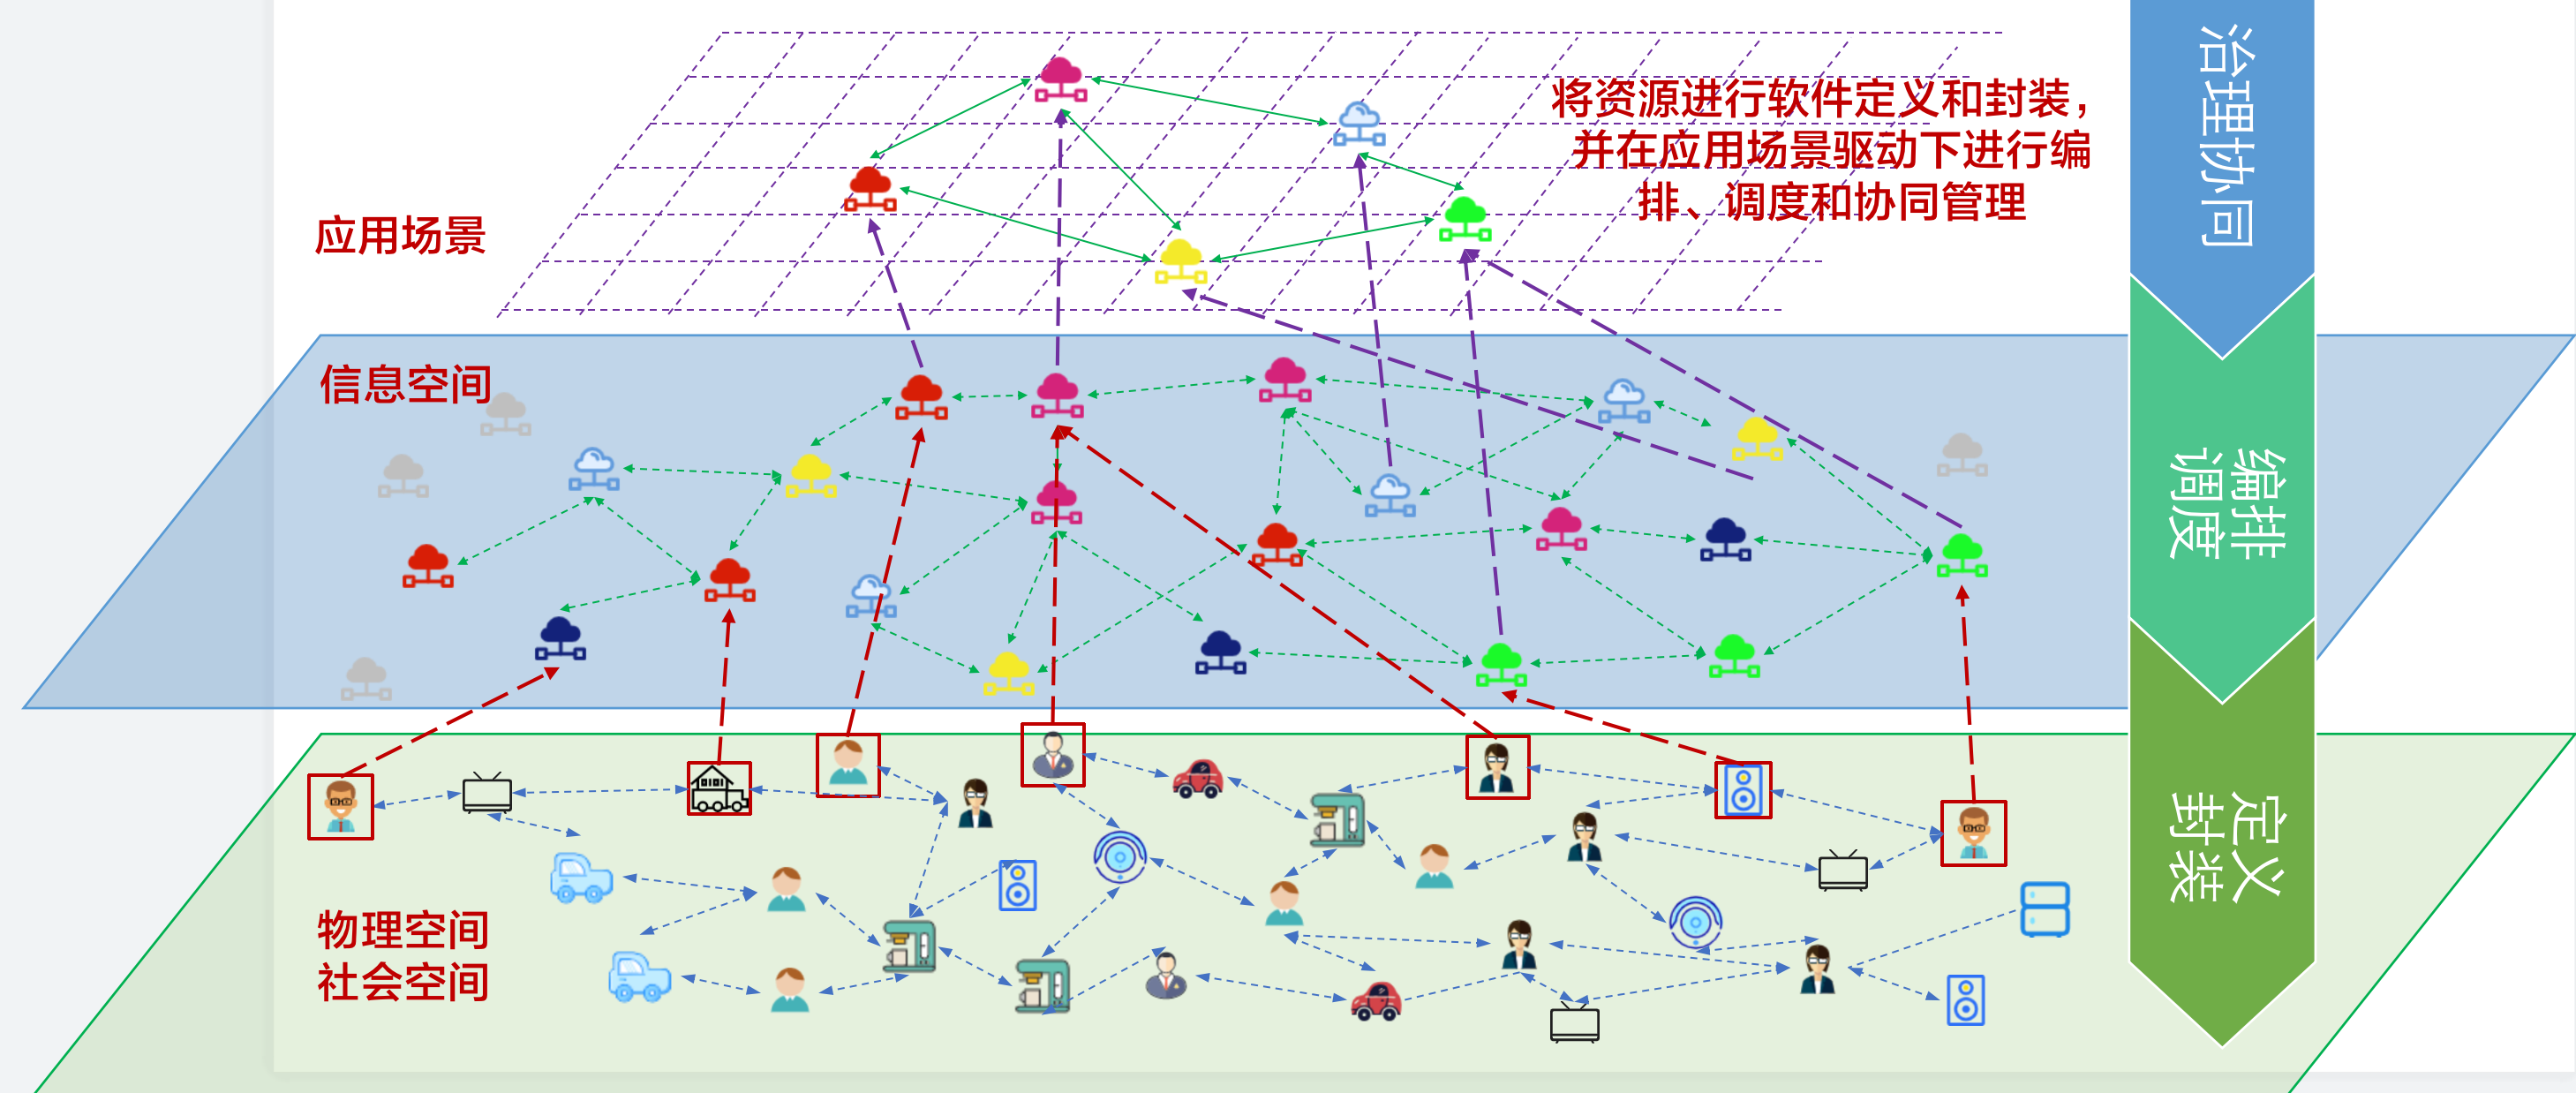
\includegraphics[width=10cm, height=5cm]{demo/blood_red_demo/p01.png}
\end{frame}

\begin{frame}{Why Microservices for IoT Applications?}
    \begin{itemize}
        \item  it is not trivial to integrate IoT devices with existing applications
        \begin{itemize}
            \item IoT applications lack a standard interface to communicate.
            \item end-users must install many applications on smart phones or computers to access IoT devices.
        \end{itemize}
        \item easy integration with existing applications and web services by uniform interface like Restful APIs 
        \item microservices' features like flexible,decoupled
    \end{itemize}
\end{frame}

\begin{frame}{Differences between web microservices and IoT microservices?}
    \begin{itemize}
        \item IoT services don't support elastic scaling 
        \item IoT services need to pair device's state  
        \item Most IoT services are spatio-temporally correlated
        \begin{itemize}
            \item spatio-temporal attribute is part of IoT devices and greatly influence end-users' experience when they use IoT devices
            \item IoT services need to provide seamless integration and dynamic interaction with the physical world, and  spatio-temporal attribute is basic feature of physical world.
        \end{itemize}
    \end{itemize}
    \begin{block}{Problem01}
    We need to provide a framework for developing IoT microservices.
    \end{block}
\end{frame}

\begin{frame}{Why a message-driven platform?}
    \begin{block}{Message-Driven (in contrast to Event-Driven)}
    \textbf{\alert{A message is an item of data that is sent to a specific destination.}} An event is a signal emitted by a component upon reaching a given state. In a message-driven system \textbf{\alert{addressable recipients await the arrival of messages and react to them, otherwise lying dormant.}}In an event-driven system notification listeners are attached to the sources of events such that they are invoked when the event is emitted. So \textbf{\alert{an event-driven system focuses on addressable event sources while a message-driven system concentrates on addressable recipients.}} (https://www.reactivemanifesto.org/glossary#Message-Driven)
    \end{block}
\end{frame}

\begin{frame}{Why a message-driven platform?}
    \textbf{ThingsBoard}
    \begin{figure}[t]                               
    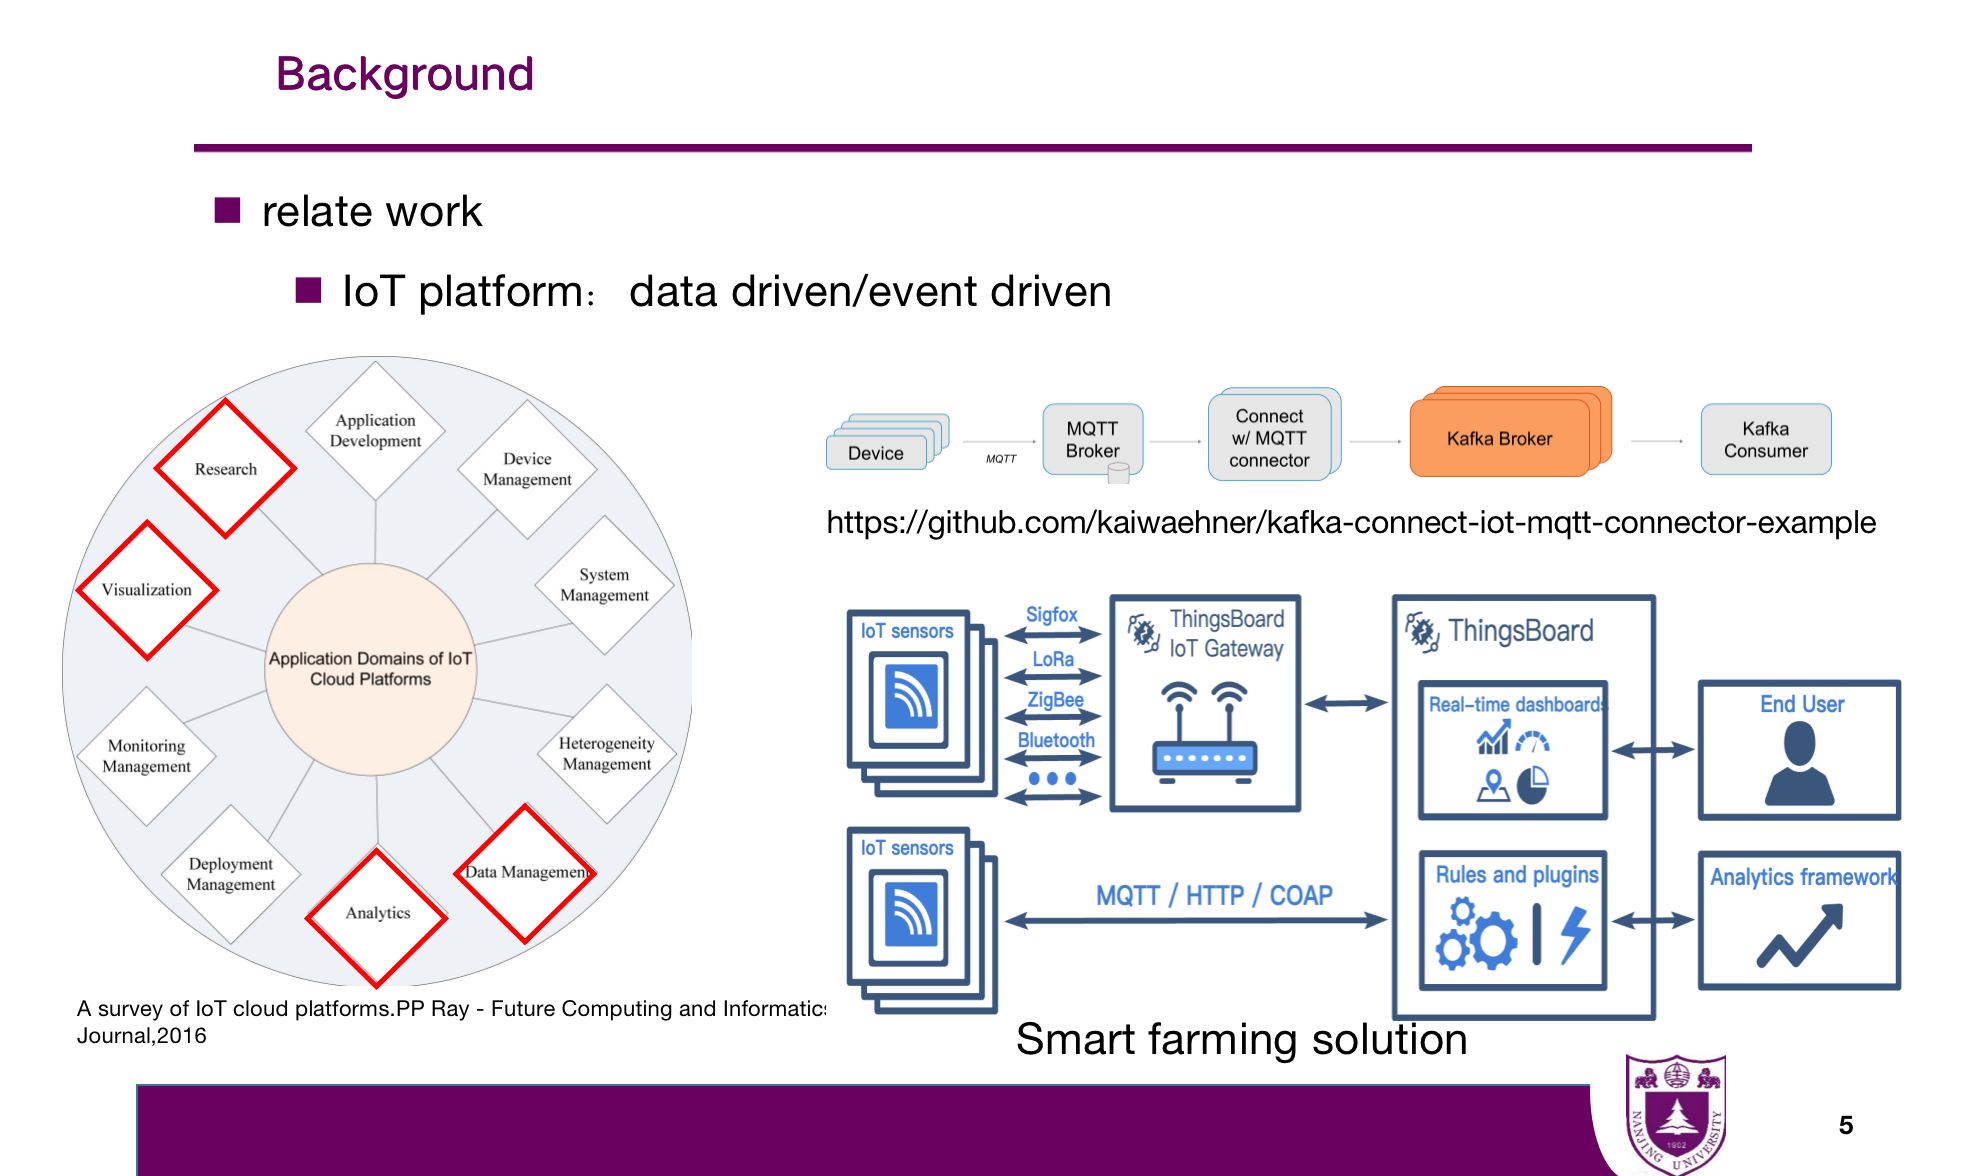
\includegraphics[width=12cm, height=7cm]{demo/blood_red_demo/IoTPlatform.png}
    \centering
    \end{figure}
\end{frame}

\begin{frame}{Why a message-driven platform?}
    \textbf{Situation-Aware IoT Service Coordination Using the
Event-Driven SOA Paradigm(TNSM'2016)}
    \begin{figure}[t]                               
    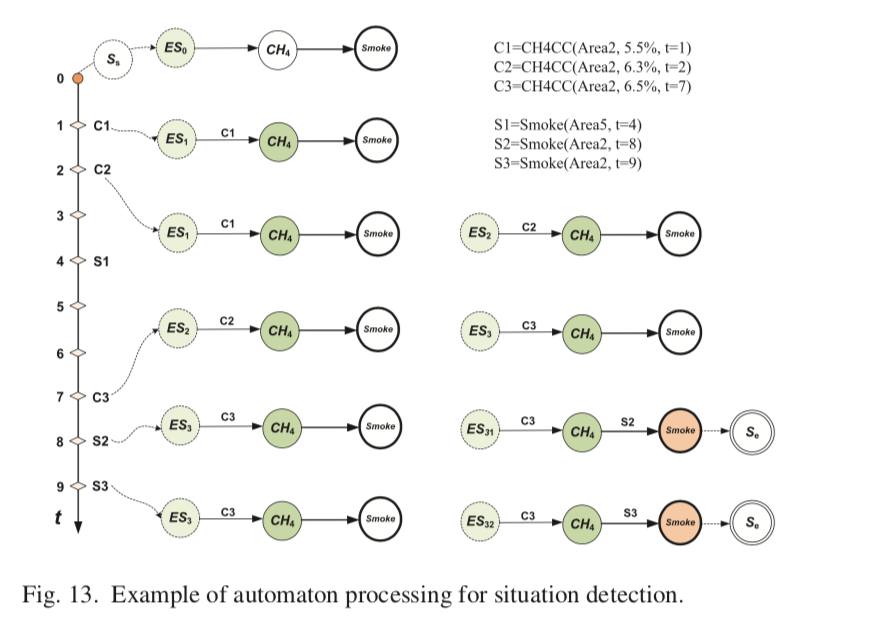
\includegraphics[width=10cm, height=6cm]{demo/blood_red_demo/edExample.png}
    \centering
    \end{figure}
\end{frame}

\begin{frame}{Why a message-driven platform?}
    \textbf{Message-driven architecture uses an asynchronous message-based Publish/Subscribe mode, which is well suited to the characteristics of the IoT, which are “high autonomy inside a domain and efficient coordination across domains.” }
     \begin{block}{Problem02}
    We need to provide a message-driven platform called ServiceMatrix.
    \end{block}
    
  \begin{block}{Problem03}
    How to Orchestrate IoT Microservices in ServiceMatrix?
    \end{block}
\end{frame}

\section{Scenario}
\begin{frame}{A smart home}
     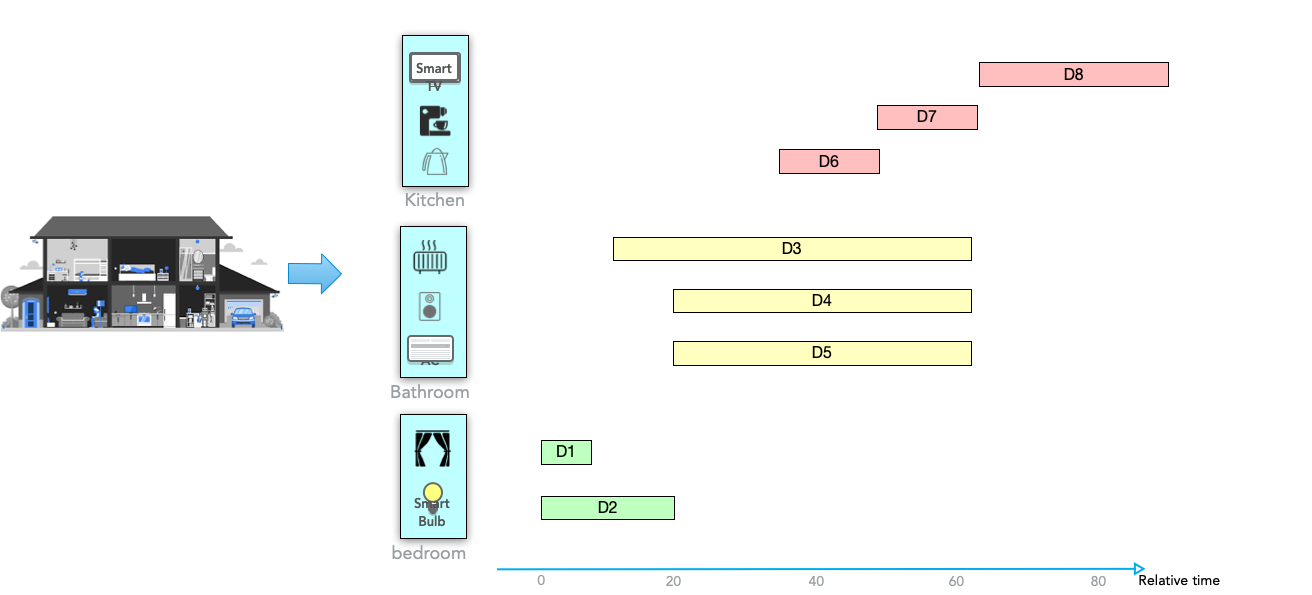
\includegraphics[width=10cm, height=5cm]{demo/blood_red_demo/scenario.png}
\end{frame}
\section{Architecture}
\begin{frame}{IoT Microservice}
    \frametitle{IoT Microservice}
    \begin{columns}
    \column{0.5\textwidth}
    \begin{itemize}
    \item restful apis for updating device's attributes
    \item annotations for Mapping messages and apis
    \end{itemize}
    
\includegraphics[width=6cm, height=1.5cm]{demo/blood_red_demo/annotation.png}
    \column{0.5\textwidth}
      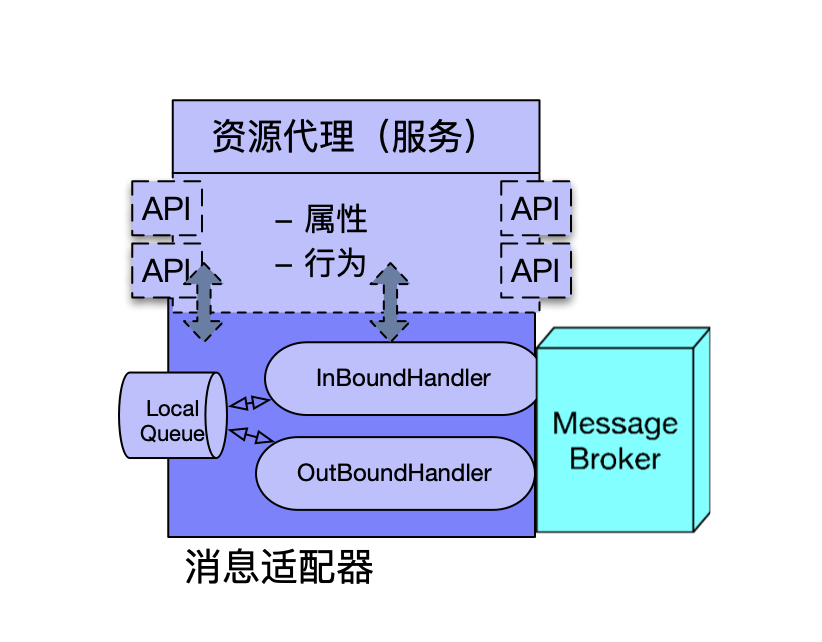
\includegraphics[width=6cm, height=5cm]{demo/blood_red_demo/microservice.png}
    \end{columns}
\end{frame}

\begin{frame}{Communication}
    \begin{block}{Definition1}
    $$ClientMessage(cm)=<id,mt,dt,ts,loc,msg>$$
    \end{block}
    \begin{itemize}
        \item \textbf{id}:serviceId(Identifier)
        \item \textbf{mt}:messageType(BIND,UNBIND,NORMAL,HEARTBEAT)
        \item \textbf{dt}:deviceType(classify devices by deviceType)
        \item \textbf{ts}:timeStamp(the time message is published)
        \item \textbf{loc}:location(device's location when message is published)
        \item \textbf{msg}:messageBody
    \end{itemize}
    $$cm = <tv1,BIND,tv,1510369871,room809,"bind to mq.">$$
    \begin{block}{Definition2}
    $$BrokerMessage(bm)=<id,mt,ts,loc,msg>$$
    \end{block}
    \begin{itemize}
        \item \textbf{mt}: messageType(ACKBIND,ACKUNBIND,ERROR,SERVER)
    \end{itemize}
\end{frame}

\begin{frame}{Communication}
    \textbf{Architecture:}
    \begin{figure}[t]
     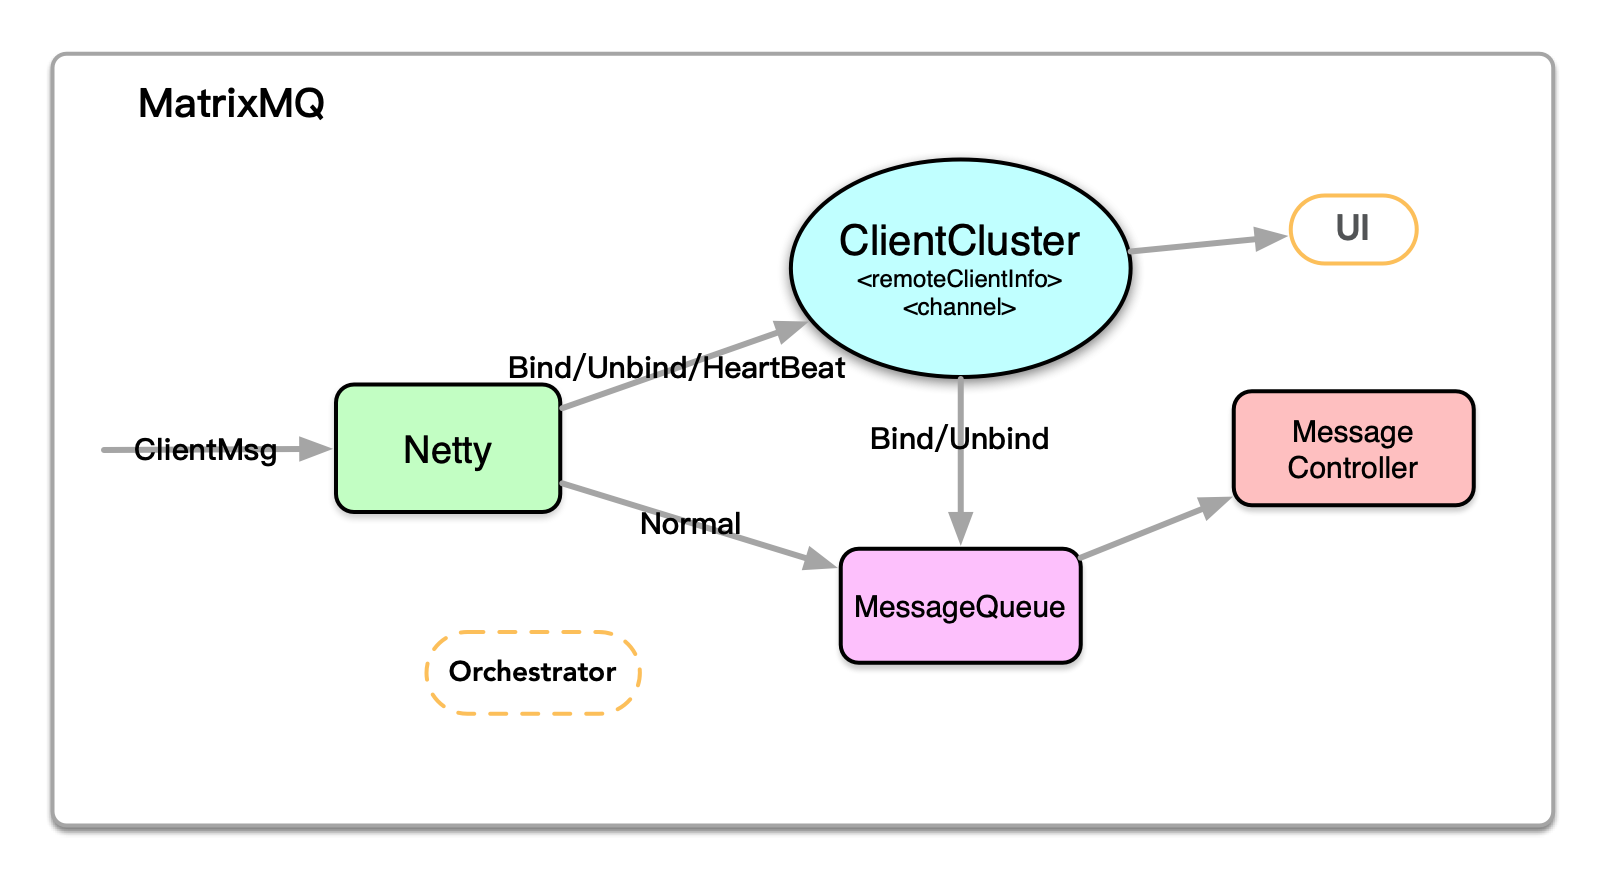
\includegraphics[width=10cm, height=5cm]{demo/blood_red_demo/matrixMQ.png}
    \centering
    \end{figure}
    
\end{frame}

\begin{frame}{Service Composition}
    \textbf{Process Example}
 \begin{figure}[t]
     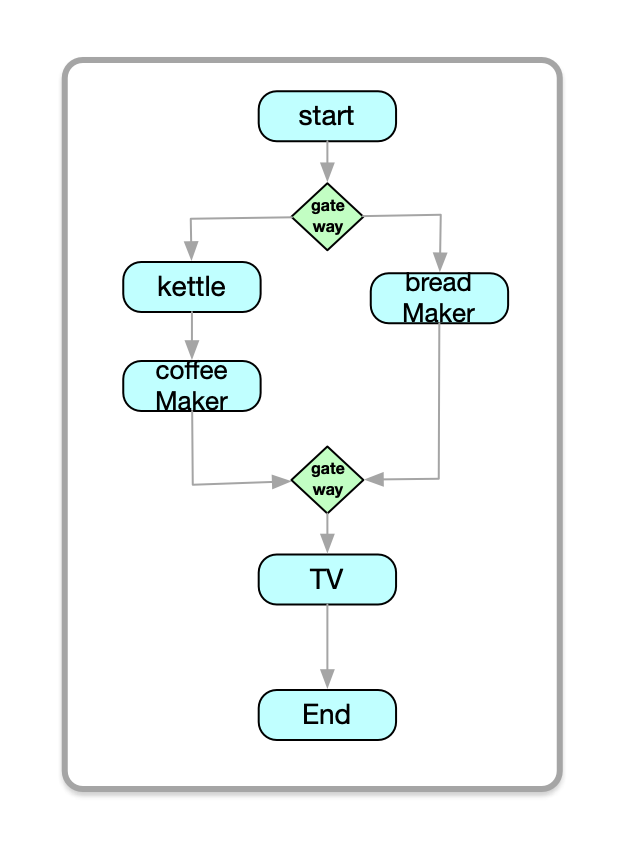
\includegraphics[width=7cm, height=8cm]{demo/blood_red_demo/kictenprocess.png}
    \centering
    \end{figure}
\end{frame}

\begin{frame}{Service Composition}
    \textbf{Related works:}
    \begin{itemize}
        \item workflow engine
        \begin{itemize}
            \item Attribute, structure and semantics based service mapping approach for collaborative business process development(TSC'2018)
        \end{itemize}
        \item GUI
        \begin{itemize}
            \item A fine-grained api link prediction approach supporting mashup recommendation(ICWS'2017)
        \end{itemize}
         \item machine learning
        \begin{itemize}
            \item A reinforcement learning method for constraint-satisfied services composition(TSC'2017)
            \item Qos constrained large scale web service composition using abstraction refinement(TSC'2017)
        \end{itemize}
    \end{itemize}
\end{frame}

\begin{frame}{Service Composition}
    \textbf{Convenience-Based Periodic Composition of IoT Services(ICSOC'2018)}
    \frametitle{Service Composition}
    \begin{columns}
    \column{0.5\textwidth}
       \begin{figure}[t]
     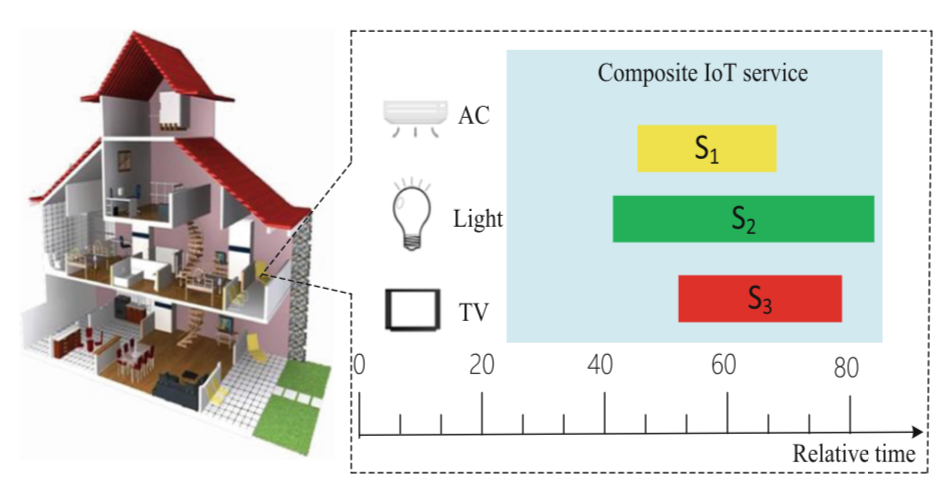
\includegraphics[width=6cm, height=4cm]{demo/blood_red_demo/compositeIoTService.png}
    \centering
    \end{figure}
    \column{0.5\textwidth}
       \begin{figure}[t]
     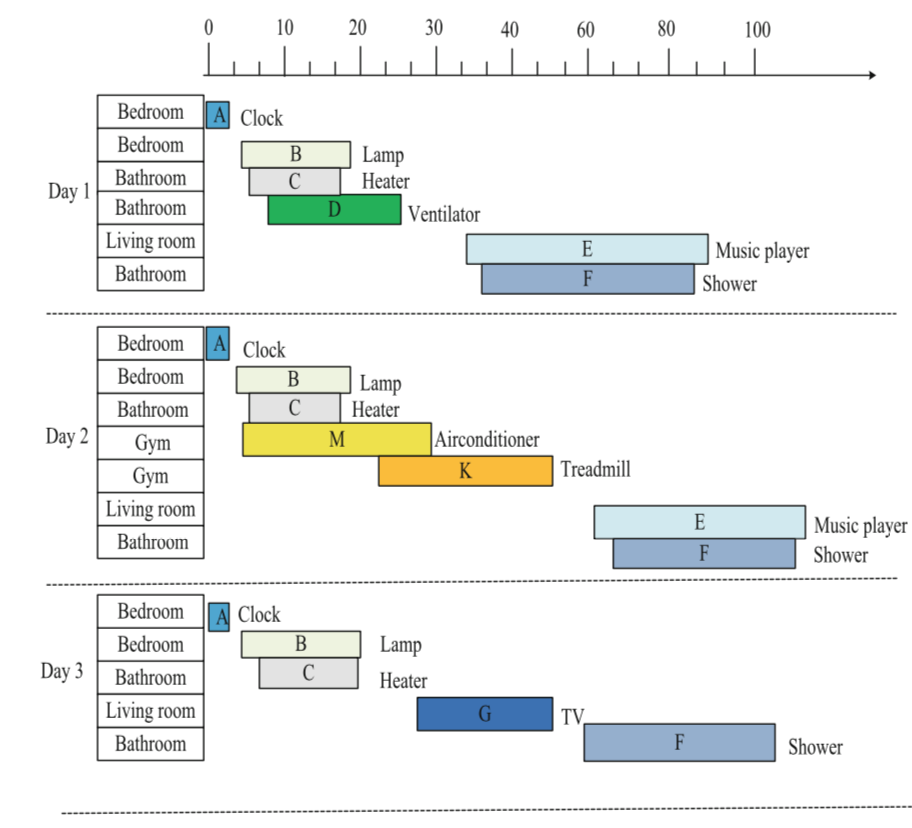
\includegraphics[width=6cm, height=4cm]{demo/blood_red_demo/compositeexample.png}
    \centering
    \end{figure}
    \end{columns}
\end{frame}

\begin{frame}{Service Composition}
    \begin{itemize}
        \item Contribution: a algorithm PCMiner(Periodic Composite IoT service Miner)
        \item Datasets: CASAS / a dataset from MIT
    \end{itemize}
    \begin{figure}[t]
    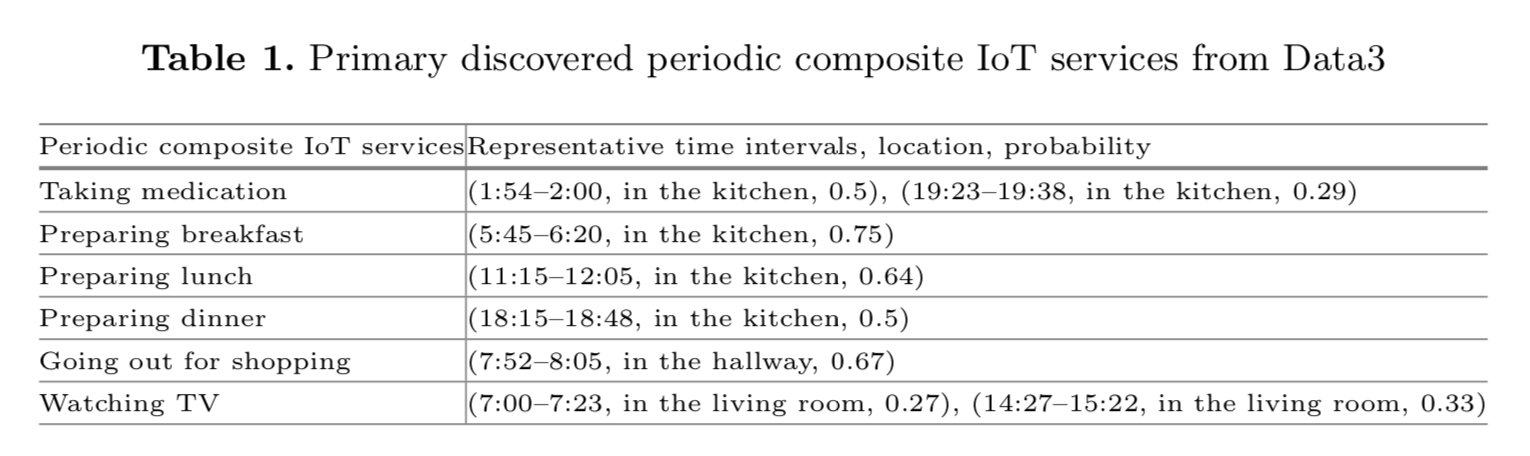
\includegraphics[width=10cm, height=4cm]{demo/blood_red_demo/results.png}
    \centering
    \end{figure}
\end{frame}

\begin{frame}{Service Composition}
    \textbf{predict periodic process}
    \begin{itemize}
        \item define process
        \item predict periodic process
    \end{itemize}
    \begin{figure}[t]
    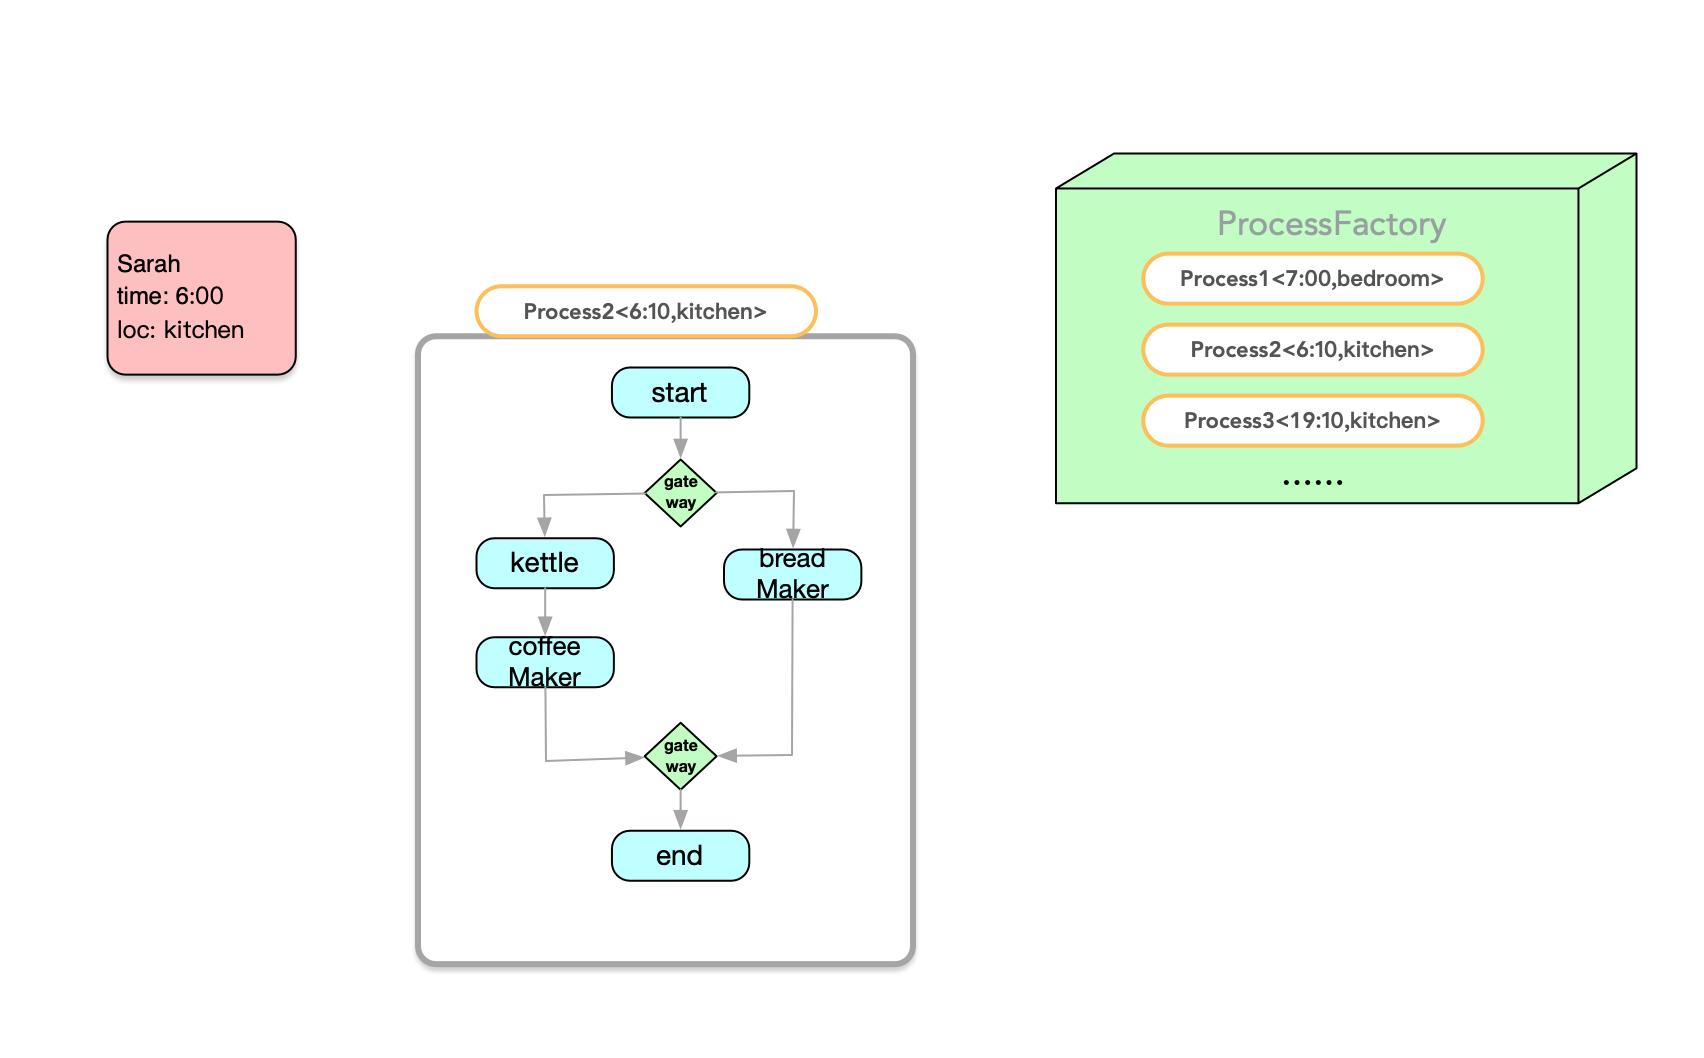
\includegraphics[width=10cm, height=5cm]{demo/blood_red_demo/periodicprocess.png}
    \centering
    \end{figure}
\end{frame}
\begin{frame}{Experiments}
    \frametitle{Datasets}
    \begin{columns}
    \column{0.5\textwidth}
    \textbf{CASAS}
    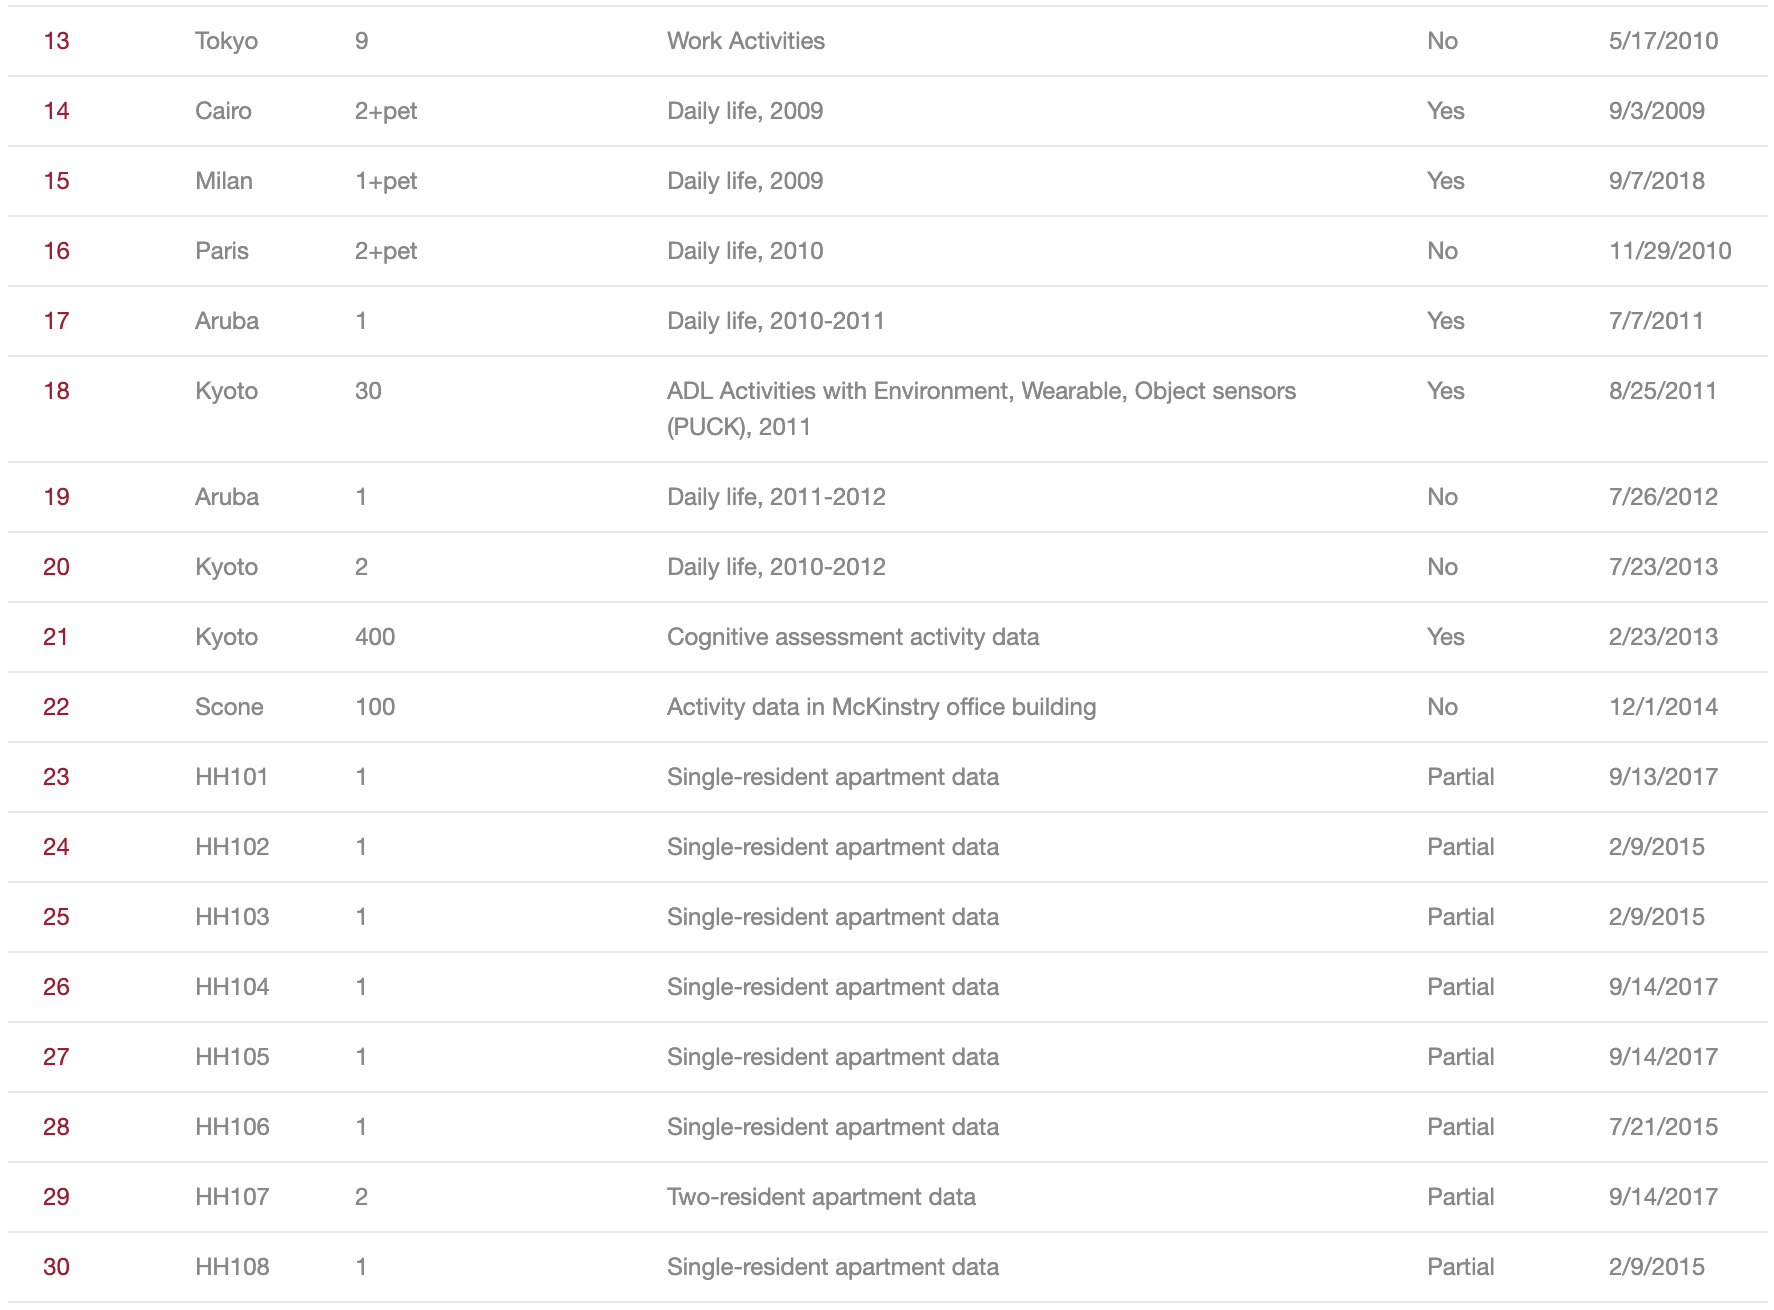
\includegraphics[width=6cm, height=5cm]{demo/blood_red_demo/CASAS.png}
    \column{0.5\textwidth}
    \textbf{Tapia}
      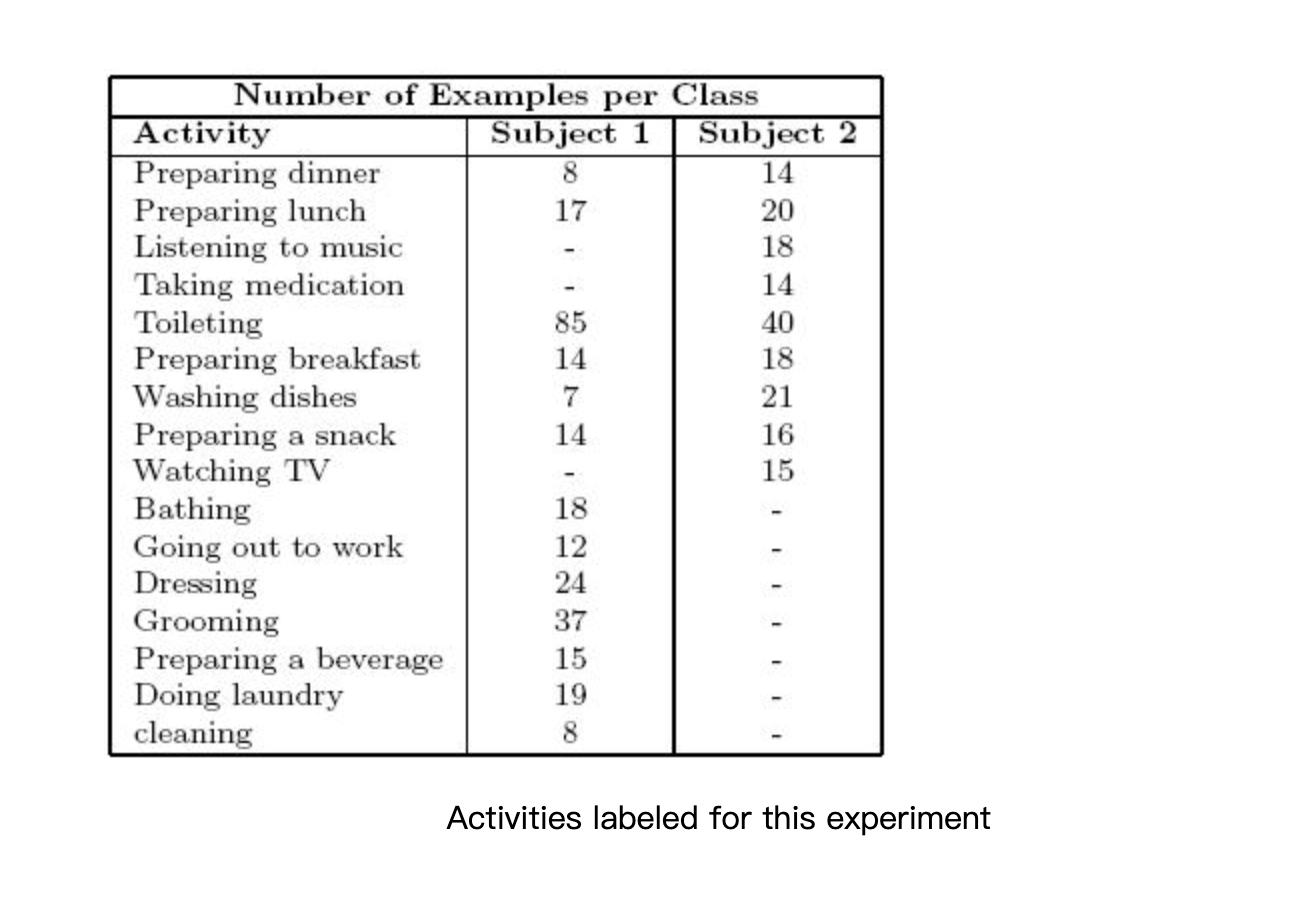
\includegraphics[width=7cm, height=5cm]{demo/blood_red_demo/Tapia.png}
    \end{columns}
\end{frame}
\section{Future work}
\begin{frame}{future work}
    \begin{itemize}
        \item predict periodic process
        \item make ServiceMatrix work
        \item do some experiments
    \end{itemize}
\end{frame}

\begin{frame}
\begin{figure}
    \centering
    
\includegraphics[width=0.9\textwidth]{demo/blood_red_demo/thanks.pdf}
\end{figure}
\end{frame}
%% normal frame


% \begin{frame}
%     \frametitle{An Example}

%     \begin{parchment}[Question]
%         Assume that a patient would like to have such a test carried out on him. The physician recommends a test which is guaranteed to detect HIV-positive whenever a patient is infected. On the other hand, for healthy patients it has a $1\%$ error rate. That is, with probability 0.01 it diagnoses a patient as HIV-positive even when he is, HIV-negative. \uwave{Moreover, assume that $0.15\%$ of the population is infected.}
%         \\[2ex]
%         Now the patient has the test carried out and the test returns HIV-negative. In this case, logic implies that he is healthy, since the test has $100\%$ detection rate. In the converse case things are not quite as straightforward.
%         \\[2ex]
%         So what's the $p(X = \mathtt{HIV+}|T = \mathtt{HIV+})$?
%     \end{parchment}
    
% \end{frame}

% \begin{frame}
%     \frametitle{An Example}

%     \center{
%     \begin{tabular}{ c | c c }
%         $p(t|x)$ & $X = \mathtt{HIV-}$ & $X=\mathtt{HIV+}$ \\
%         \hline
%         $T=\mathtt{HIV-}$ & 0.99 & 0 \\
%         $T=\mathtt{HIV+}$ & 0.01 & 1
%     \end{tabular}
%     }

%     $$
%     p(X = \mathtt{HIV+}) = 0.0015
%     $$
% \end{frame}

% \begin{frame}
%     \frametitle{An Example}

%     By Bayes rule we may write
%     $$
%     p(X = \mathtt{HIV+}|T=\mathtt{HIV+}) = \frac{p(T=\mathtt{HIV+}|X=\mathtt{HIV+})p(X=\mathtt{HIV+})}{p(T=\mathtt{HIV+})}
%     $$

%     While we know all terms in the numerator, $p(T = \mathtt{HIV+})$itself is unknown. That said, it can be computed via
%     \begin{align}
%     \nonumber p(T=\mathtt{HIV+}) &= \sum_{x \in \{\mathtt{HIV+}, \mathtt{HIV-}\}}p(T=\mathtt{HIV+},x) \\
%     \nonumber &= \sum_{x \in \{\mathtt{HIV+}, \mathtt{HIV-}\}}p(T=\mathtt{HIV+}|x)p(x) \\
%     \nonumber &= 1.0 \cdot 0.0015 + 0.01 \cdot 0.9985
%     \end{align}

%     Substituting back into the conditional expression yields
%     $$
%     p(X = \mathtt{HIV+}|T=\mathtt{HIV+}) = \frac{1.0 \cdot 0.0015}{1.0 \cdot 0.0015 + 0.01 \cdot 0.9985} = 0.1306
%     $$

% \end{frame}


% \begin{frame}
%     \frametitle{How can we improve the diagnosis}

%     % Define block styles
%     \tikzset{
%         grayCircle/.style = {
%             draw,
%             circle,
%             node distance=2.5cm,
%             minimum size=1.5cm,
%             fill=black!20
%         }
%     }

%     \center
%     \begin{tikzpicture}
%         \node[grayCircle] (age) {age};
%         \node[grayCircle, right of=age, style={fill=none}] (x) {x};
%         \node[grayCircle, right of=x, yshift=1.25cm] (t1) {test 1};
%         \node[grayCircle, below of=t1] (t2) {test 2};
%         \draw[->, >=latex] (age) -- (x);
%         \draw[->, >=latex] (x) -- (t1);
%         \draw[->, >=latex] (x) -- (t2);
%     \end{tikzpicture}

%     \begin{figure}
%         \caption{A graphical description of our HIV testing scenario. Knowing the age of the patient influences our prior on whether the patient is HIV positive (the random variable X). The outcomes of the tests 1 and 2 are independent of each other given the status X. We observe the shaded random variables (age, test 1, test 2) and would like to infer the un-shaded random variable X.}
%     \end{figure}

% \end{frame}


% \begin{frame}
%     \frametitle{How can we improve the diagnosis}

%     \begin{parchment}[Including additional observed random variables]
%     One way is to obtain further information about the patient and to use this in the diagnosis. For instance, information about his age is quite useful. Suppose the patient is 35 years old. In this case we would want to compute $p(X = \mathtt{HIV+}|T = \mathtt{HIV+}, A = 35)$ where the random variable A denotes the age.
%     \end{parchment}

%     The corresponding expression yields:
%     $$
%     \frac{p(T=\mathtt{HIV+}|X=\mathtt{HIV+},A)p(X=\mathtt{HIV+}|A)}{p(T=\mathtt{HIV+}|A)}
%     $$
% \end{frame}


% \begin{frame}
%     \frametitle{How can we improve the diagnosis}

%     We may assume that the test is independent of the age of the patient, i.e.
%     $$
%     p(t|x,a) = p(t|x)
%     $$

%     What remains therefore is $p(X = \mathtt{HIV+}|A)$. Recent US census data pegs this number at approximately $0.9\%$. 
%     \begin{align}
%     \nonumber & p(X = \mathtt{H+}|T = \mathtt{H+}, A) = \frac{p(T=\mathtt{H+}|X=\mathtt{H+},A)p(X=\mathtt{H+}|A)}{p(T=\mathtt{H+}|A)} \\
%     \nonumber &= \frac{p(T=\mathtt{H+}|X=\mathtt{H+},A)p(X=\mathtt{H+}|A)}{p(T=\mathtt{H+}|X=\mathtt{H+},A)p(X=\mathtt{H+}|A) + p(T=\mathtt{H+}|X=\mathtt{H-},A)p(X=\mathtt{H-}|A)} \\
%     \nonumber & = \frac{p(T=\mathtt{H+}|X=\mathtt{H+})p(X=\mathtt{H+}|A)}{p(T=\mathtt{H+}|X=\mathtt{H+})p(X=\mathtt{H+}|A) + p(T=\mathtt{H+}|X=\mathtt{H-})p(X=\mathtt{H-}|A)} \\
%     \nonumber & = \frac{1 \cdot 0.009}{1 \cdot 0.009 + 0.01 \cdot 0.991} = 0.48
%     \end{align}

% \end{frame}


% \begin{frame}
%     \frametitle{How can we improve the diagnosis}

%     \begin{parchment}[Multiple measurements]
%     A second tool in our arsenal is the use of multiple measurements. After the first test the physician is likely to carry out a second test to confirm the diagnosis. We denote by $T_1$ and $T_2$ (and $t_1$,$t_2$ respectively) the two tests. Obviously, what we want is that $T_2$ will give us an "independent" second opinion of the situation.
%     \\[2ex]
%     What we want is that the diagnosis of $T_2$ is independent of that of $T_2$ given the health status X of the patient. This is expressed as
%     $$
%     p(t_1,t_2|x) = p(t_1|x)p(t_2|x)
%     $$
%     which are commonly referred to as \uwave{conditionally independent}.

%     \end{parchment}
% \end{frame}

% \begin{frame}
%     \frametitle{How can we improve the diagnosis}

%     we assume that the statistics for $T_2$ are given by
%     \center{
%     \begin{tabular}{ c | c c }
%         $p(t_2|x)$ & $X = \mathtt{HIV-}$ & $X=\mathtt{HIV+}$ \\
%         \hline
%         $T_2=\mathtt{HIV-}$ & 0.95 & 0.01 \\
%         $T_2=\mathtt{HIV+}$ & 0.05 & 0.99 
%     \end{tabular}
%     }

%     \flushleft
%     for $t_1 = t_2 = \mathtt{HIV+}$ we have
%     \begin{align}
%     \nonumber & p(X=\mathtt{H+}|T_1=\mathtt{H+},T_2=\mathtt{H+}) \\
%     \nonumber &= \frac{p(T_1=\mathtt{H+}, T_2=\mathtt{H+}|X=\mathtt{H+})p(X=\mathtt{H+}|A)}{p(T_1=\mathtt{H+}, T_2=\mathtt{H+}|A)} \\
%     \nonumber &= p(T_1=\mathtt{H+}|X=\mathtt{H+})p(T_2=\mathtt{H+}|X=\mathtt{H+})p(X=\mathtt{H+}|A) \;/ \\
%     \nonumber & p(T_1=\mathtt{H+}|X=\mathtt{H+})p(T_2=\mathtt{H+}|X=\mathtt{H+})p(X=\mathtt{H+}|A) \\
%     \nonumber & + p(T_1=\mathtt{H+}|X=\mathtt{H-})p(T_2=\mathtt{H+}|X=\mathtt{H-})p(X=\mathtt{H-}|A) \\
%     % \nonumber & p(T_{1,H+}|X_{H+})p(T_{2,H+}|X_{H+})p(X_{H+}|A) \\
%     % \nonumber & + p(T_{1,H+}|X_{H-})p(T_{2,H+}|X_{H-})p(X_{H-}|A) \\
%     \nonumber &= \frac{1 \cdot 0.99 \cdot 0.009}{1 \cdot 0.99 \cdot 0.009 + 0.01 \cdot 0.05 \cdot 0.991} = 0.95
%     \end{align}
% \end{frame}


\end{document}